% This file was created by matplotlib2tikz v0.6.15.
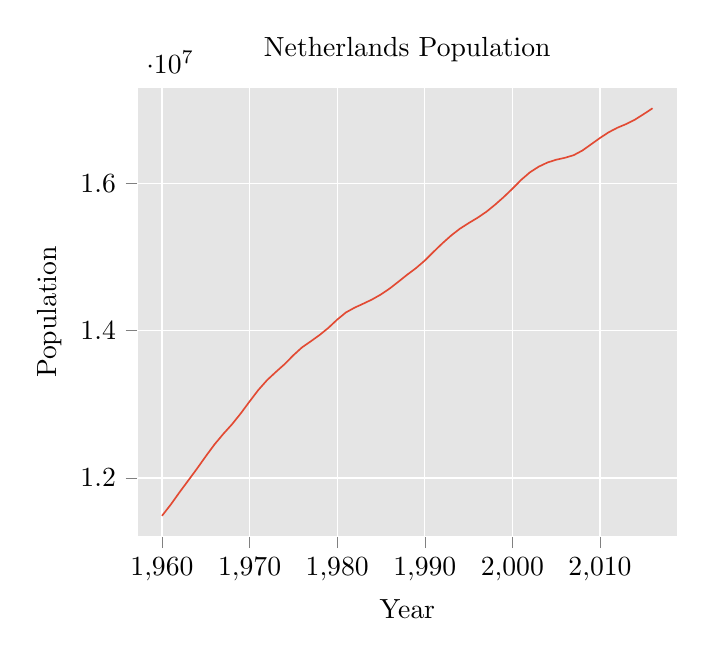
\begin{tikzpicture}

\definecolor{color0}{rgb}{0.886274509803922,0.290196078431373,0.2}

\begin{axis}[
title={Netherlands Population},
xlabel={Year},
ylabel={Population},
xmin=1957.2, xmax=2018.8,
ymin=11210042.15, ymax=17294996.85,
tick align=outside,
tick pos=left,
xmajorgrids,
x grid style={white},
ymajorgrids,
y grid style={white},
axis line style={white},
axis background/.style={fill=white!89.80392156862746!black}
]
\addplot [semithick, color0, forget plot]
table {%
1960 11486631
1961 11638712
1962 11805689
1963 11965966
1964 12127120
1965 12294732
1966 12456251
1967 12598201
1968 12729721
1969 12877984
1970 13038526
1971 13194497
1972 13328593
1973 13439322
1974 13545056
1975 13666335
1976 13774037
1977 13856185
1978 13941700
1979 14038270
1980 14149800
1981 14247208
1982 14312690
1983 14367070
1984 14424211
1985 14491632
1986 14572278
1987 14665037
1988 14760094
1989 14848907
1990 14951510
1991 15069798
1992 15184166
1993 15290368
1994 15382838
1995 15459006
1996 15530498
1997 15610650
1998 15707209
1999 15812088
2000 15925513
2001 16046180
2002 16148929
2003 16225302
2004 16281779
2005 16319868
2006 16346101
2007 16381696
2008 16445593
2009 16530388
2010 16615394
2011 16693074
2012 16754962
2013 16804432
2014 16865008
2015 16939923
2016 17018408
};
\end{axis}

\end{tikzpicture}